\documentclass{article}

\usepackage[utf8]{inputenc}
\usepackage{amsmath, enumitem, url}
\usepackage{xcolor}
\usepackage[margin=1in]{geometry}

% For figures.
% Package float, adds the H option which forces figure placement.
% \usepackage[demo]{graphicx}
\usepackage{graphicx, float, subfig}
\graphicspath{ {./figures/} }

\newcommand\todo{\textcolor{red}{\textbf{[TODO:] }}}

\title{Learning end-to-end control for duckiebot driving}
\author{Group: Dropouts}
\date{June 2021}

\begin{document}
\maketitle

\section{Group Information}

Members:
\begin{itemize}
    \item Keyan Pishdadian (keyanp@cs.washington.edu)
    \item Jakub Filipek (balbok@cs.washington.edu)
    \item Kyle Deeds (kdeeds@cs.washington.edu)
\end{itemize}

\noindent Source code for behavior cloning approach:
\newline
\url{https://github.com/keyan/duckiebot_behavior_cloning}

\noindent Source code for reinforcement learning approach:
\newline
\url{https://github.com/balbok0/cse571-sp21-project-2-dropouts}

\section{Task Overview}

In this project we sought to explore methods for learning an end-to-end control policy that would allow the duckiebot to navigate tracks autonomously. Our goal was to enable the duckiebot and have it navigate around an entire track without any major driving infractions (defined as exiting the lane or going off the road), using only monocular camera data. Ideally this system would be robust enough to generalize to new tracks and work on the real robot as well as in simulation.

Inspired by previous efforts in learning end-to-end control for driving using deep reinforcement learning \cite{DBLP:journals/corr/abs-1807-00412} our original plan was to evaluate a selection of reinforcement learning algorithms to solve this task. Knowing that reproducing reinforcement results is difficult and often unsuccessful \cite{henderson2019deep}, we planned to also experiment with a behavior cloning approach inspired by prior work from NVIDIA where a convolutional neural network was trained to steer a car using only image data \cite{DBLP:journals/corr/BojarskiTDFFGJM16}.

\section{Environment Setup}

We performed experimentation and evaluation of our agents in simulation and on the real robot primarily relying on the ``AI Driving Olympics" infrastructure \cite{zilly2019ai}. Our agent was structured into the AIDO submission format and then executed either in simulation or on the real duckiebot. We used the default episode length configuration, which runs agents for 60 seconds. The AIDO submission format requires structuring an agent that obeys the AIDO agent interface and accepts image observations and outputs control commands. We referenced the baseline implementations for both reinforcement learning and behavior cloning submission types, \url{https://github.com/duckietown/challenge-aido_LF-baseline-RL-sim-pytorch} and \url{https://github.com/duckietown/challenge-aido_LF-baseline-behavior-cloning}, respectively.

\subsection{Simulation}

We used the \texttt{gym-duckietown} simulator \cite{gym_duckietown} for training and evaluation of agents when using a reinforcement learning approach, as well as for evaluation when using behavior cloning (through the AIDO submission infrastructure). For reinforcement learning we only ran evaluation on the most simple map type, ``loop\_empty", which is an square map with no obstacles. Evaluations for behavior cloning used a specific ``challenge", \texttt{aido-LF-sim-validation} which runs the agent on a static selection of maps and ranks submissions against other users.

\subsection{Real World}

Evaluation on the real duckiebot was done on five different maps (\ref{fig:maps}), with a 60 second maximum episode duration. Only map2 was used for training data collection.

\begin{figure}[H]
\centering
    \subfloat[\centering map1]{{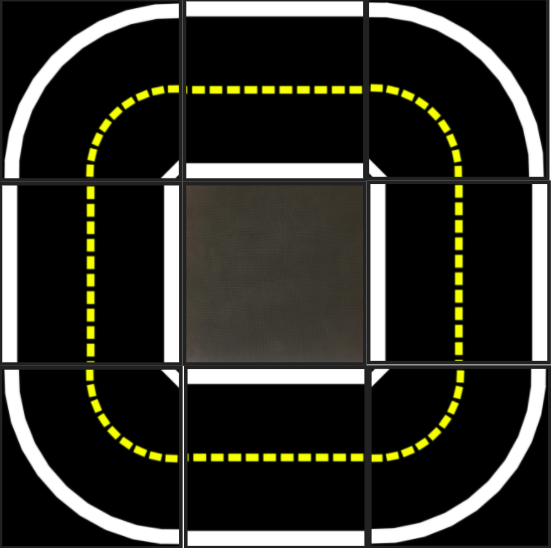
\includegraphics[width=5cm]{map1} }}
    \qquad
    \subfloat[\centering map2]{{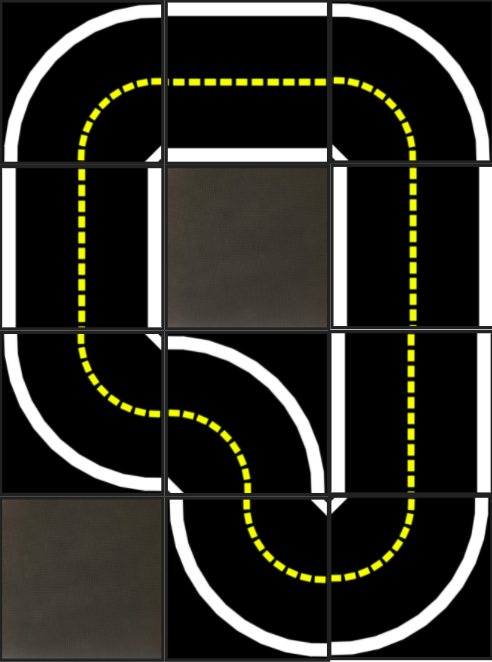
\includegraphics[width=5cm]{map2} }}
    \qquad
    \subfloat[\centering map3]{{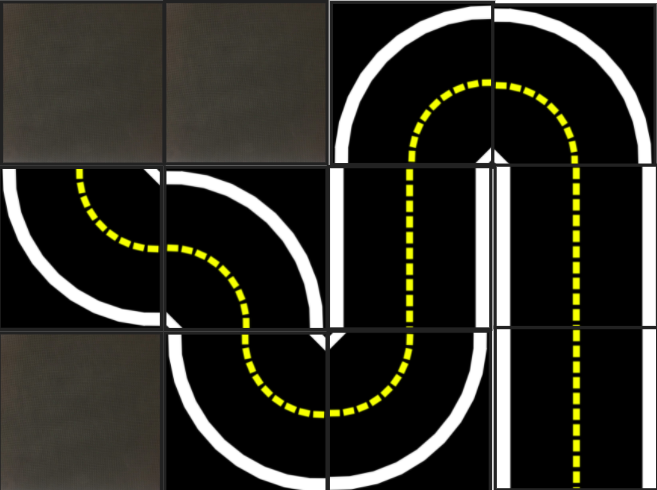
\includegraphics[angle=90,width=4cm]{map3} }}
    \qquad
    \subfloat[\centering map4]{{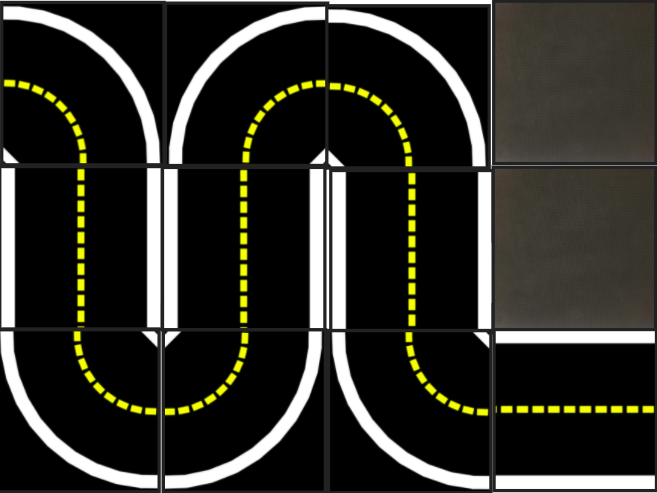
\includegraphics[angle=90,width=4cm]{map4} }}
    \qquad
    \subfloat[\centering map5]{{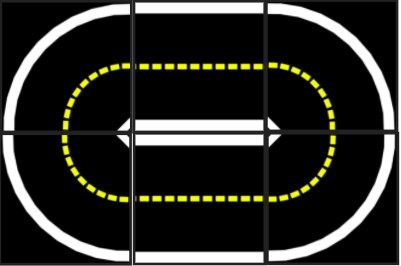
\includegraphics[angle=90,width=4cm]{map5} }}
    \qquad
    \caption{Digital overview of the five maps used for real-world evaluation.}
    \label{fig:maps}
\end{figure}

\begin{figure}[H]
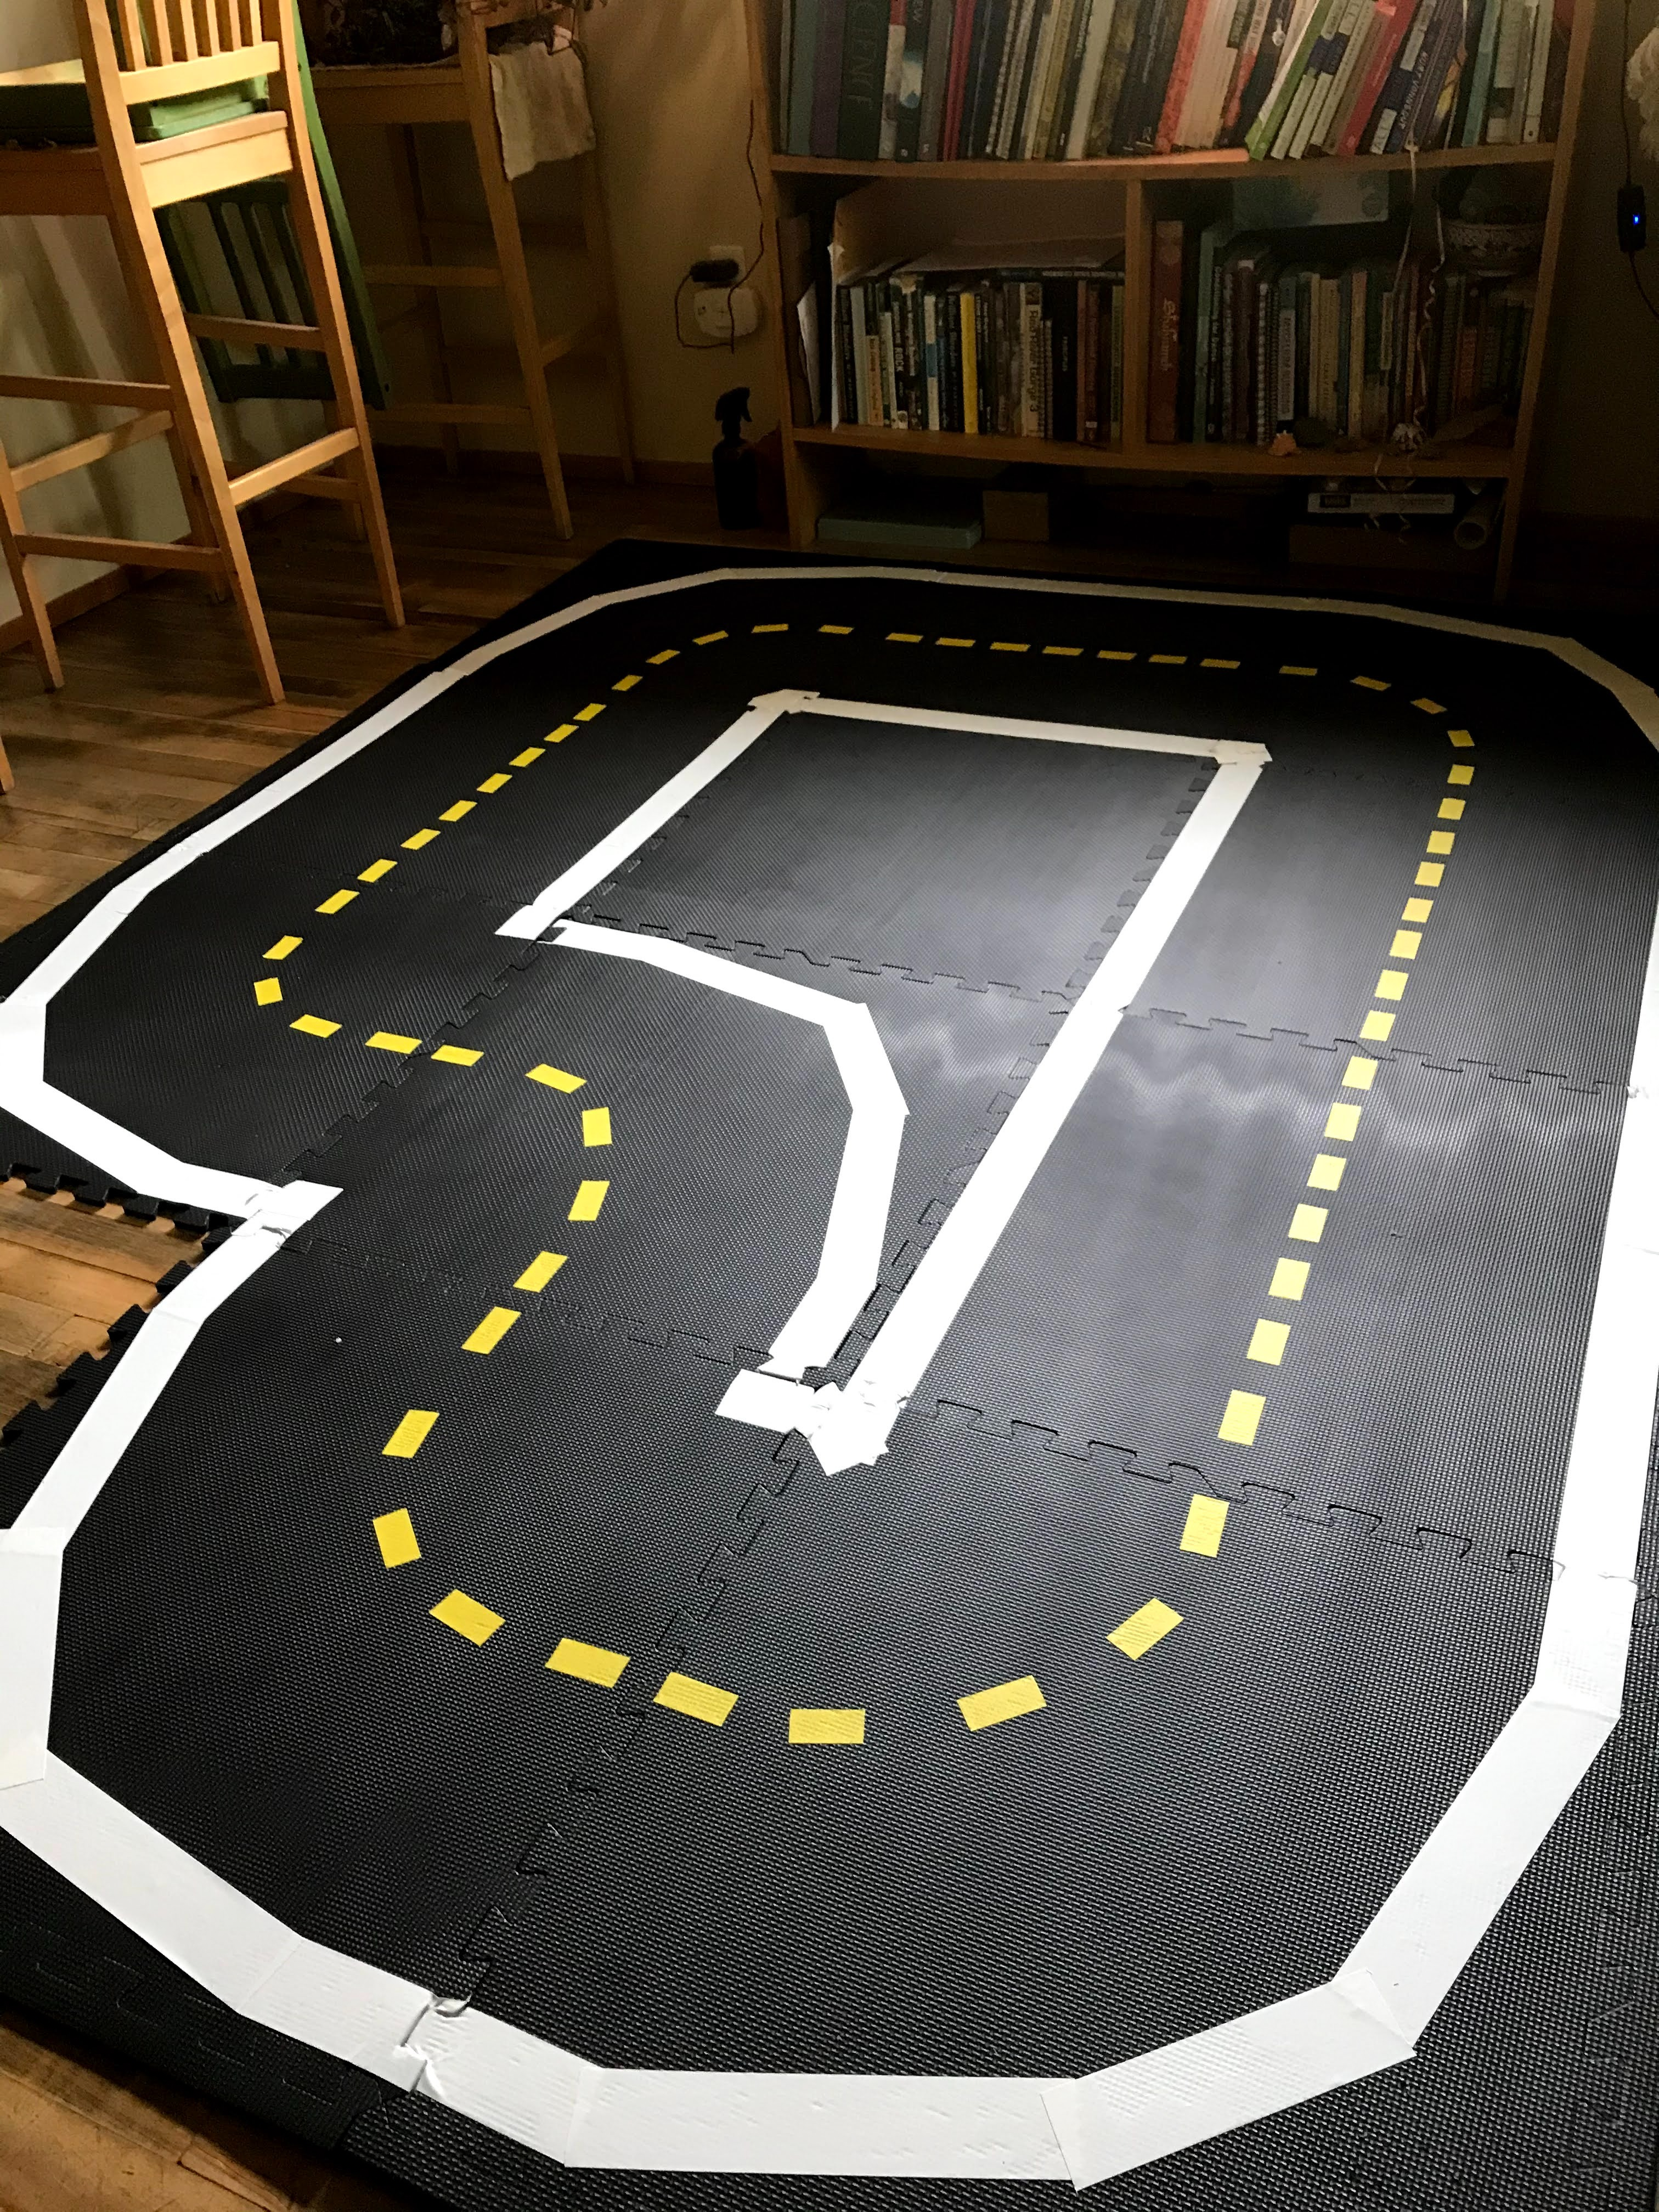
\includegraphics[width=8cm,keepaspectratio]{map2_real}
\centering
\caption{Photo of physical layout of map2.}
\label{fig:map2_real}
\end{figure}

\section{Reinforcement Learning Approach}

Our initial solution was to use the \texttt{gym-duckietown} environment to train an agent using a model-free off-policy Q-learning algorithm, for which we explored both DQN \cite{DBLP:journals/corr/MnihKSGAWR13} and DDPG \cite{journals/corr/LillicrapHPHETS15} algorithms. Our training code leveraged pre-written implementations of both algorithms provided through the RLLib package \cite{DBLP:journals/corr/abs-1712-09381}. We leveraged the existing default reward function provided by the gym environment (\url{https://git.io/JGnsg}) which is a linear function of the robot speed, position within the lane relative to the right line, and proximity to obstacles.

\todo Some brief amount of discussion about DQN and DDPG that shows we at least understand it \\

Unfortunately we were unsuccessful in achieving reasonable training results with this method, with our agent consistently showing an inability to increase average reward obtained despite experimenting with domain randomization in the simulator, training across multiple maps, and performing hyperparameter search (Figure \ref{fig:rl_training}). Our initial impression was that training an agent to perform well in simulation would be straightforward and the main challenge would be in transferring the agent to the real environment. When our agents failed to show any promising results during training and subsequently failed to perform in simulation at all, we decided to abandon this approach. Videos of evaluation of these agents in simulation can be found at:
\begin{itemize}
    \item DQN agent: \url{https://youtu.be/SDZ59_2zhGg}
    \item DDPG agent: \url{https://youtu.be/1xL8b2MK6N4}
\end{itemize}

\begin{figure}[H]
\centering
    \subfloat{{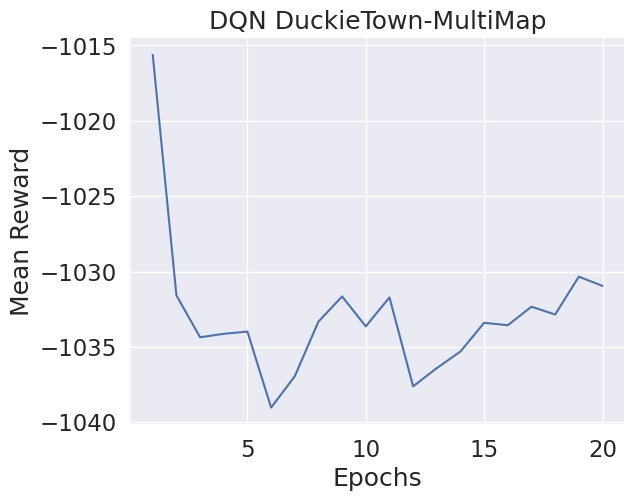
\includegraphics[width=7cm]{dqn_reward} }}
    \qquad
    \subfloat{{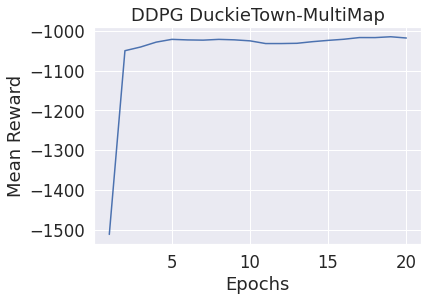
\includegraphics[width=7cm]{ddpg_reward} }}
    \caption{Mean reward obtained per epoch during training of the DQN (a) and DDPG (b) solutions. Both solutions failed to improve mean reward. Here only 20 epochs are shown, but the plateau in reward obtained was observed even when trained for many more epochs.}
    \label{fig:rl_training}
\end{figure}

\section{Behavior Cloning Approach}

Our focus then shifted towards a strategy where we would train a convolutional neural network (CNN) that would accept a single camera image from the robot at each timestep and then output a prediction for the linear and angular velocity that the robot should apply. This approach was influenced by work from NVIDIA where this technique was applied to predicting a single value representing the steering of the vehicle \cite{DBLP:journals/corr/BojarskiTDFFGJM16}. We designed several CNN models (discussed in Section \ref{sec:model_arch}) and trained them on a combination of simulation and real world data, then evaluated these models using the AIDO leaderboard and on the real duckiebot. An high-level overview of this system is shown in Figure \ref{fig:cnn_overview}.

\begin{figure}
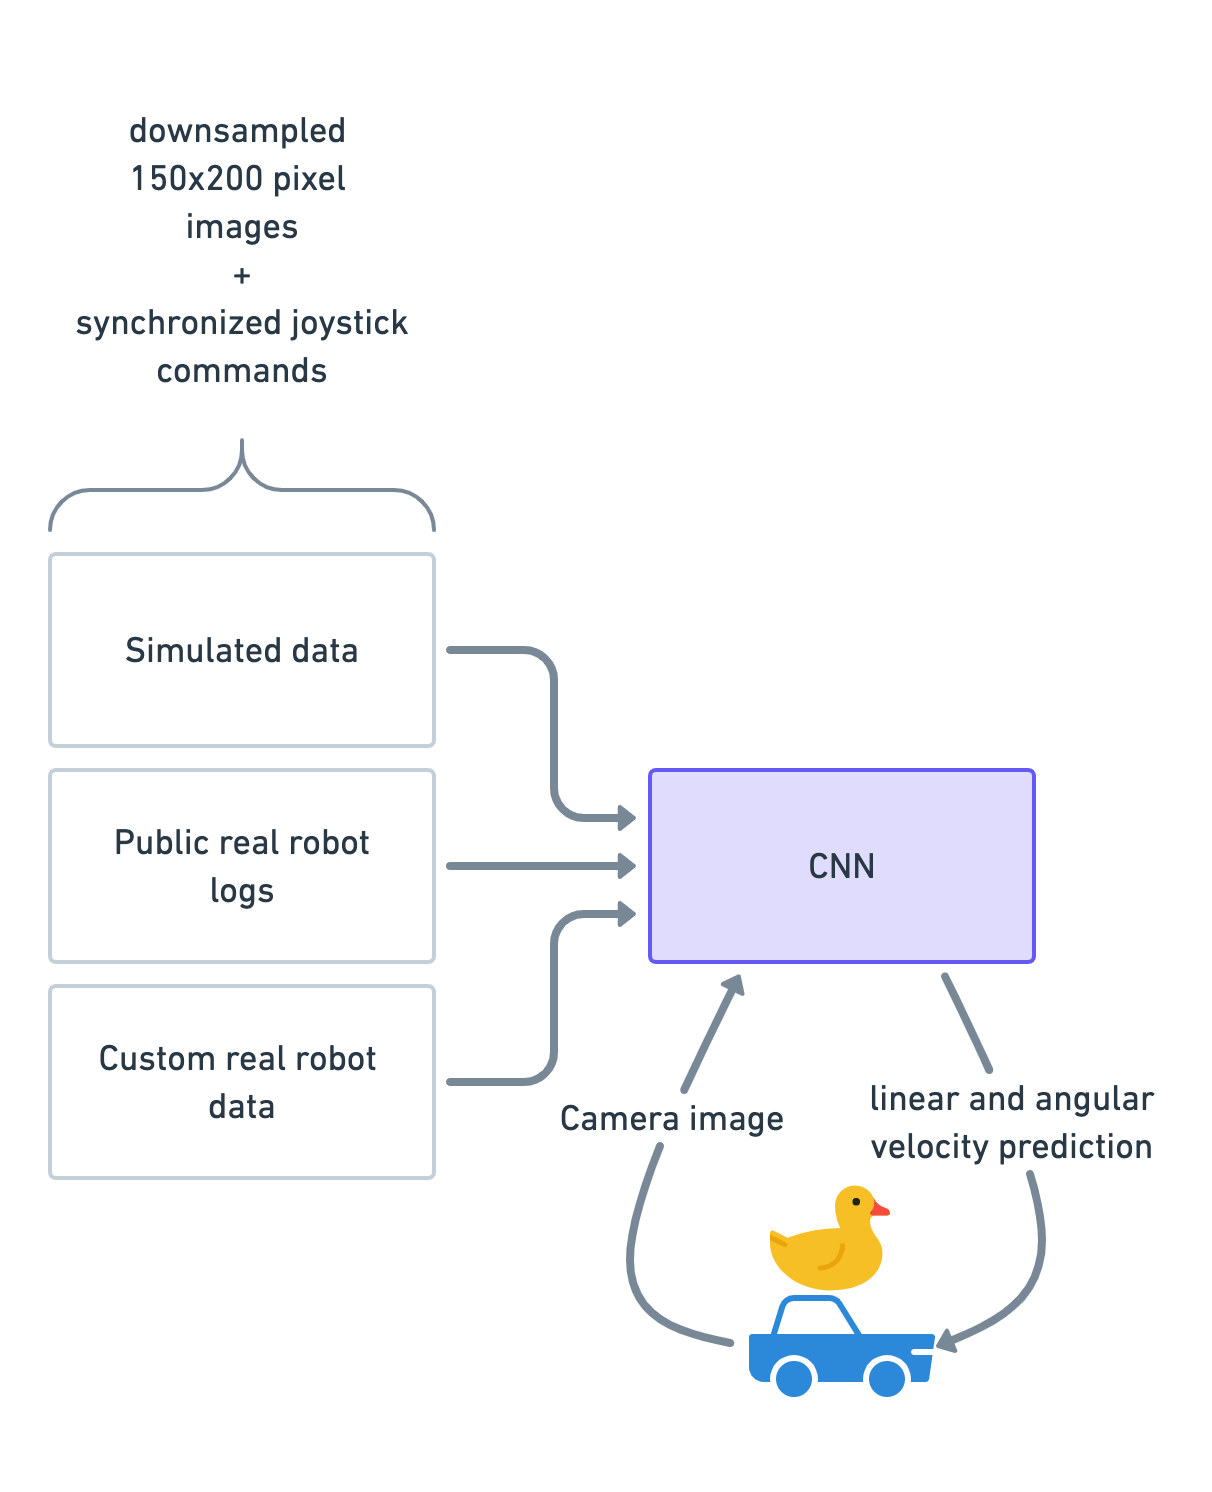
\includegraphics[width=8cm,keepaspectratio]{cnn_overview}
\centering
\caption{Overview of input training data and data flow during inference for the behavior cloning approach to end-to-end control. At runtime the robot passes each observation frame to the CNN model to produce predicted linear and angular velocities. These velocities are converted to left and right wheel velocity commands which are issued to the robot.}
\label{fig:cnn_overview}
\end{figure}

\subsection{Data Preparation}

Data collection from simulation in the \texttt{gym-duckietown} environment is easier, faster, and less noisy than real world data, so the overall data strategy was to focus on collecting a large volume of simulated data and augmenting its applicability to real robot evaluation by including a smaller amount of real robot data extracted from ROS bags.

To collect simulated data, a built-in demo was executed in the simulator that uses a pure pursuit controller \cite{DBLP:journals/corr/PadenCYYF16} to geometrically determine the optimal robot controls, the resulting image observations and joystick controls were aggregated. Image observations from simulation were downsampled to 150x200 and domain randomization was applied during the simulation runs to help prevent overfitting to the simulation environment.

Real robot data was collected through a combination of accessing publicly available ROS bags \cite{paull17duckietown} and ROS bags recorded from demonstrations with one of our own robots on map2 (Figure \ref{fig:maps}b). When selecting public robot logs, we attempted to find executions which were successfully navigating the map, were free of obstacles, and contained turns. For the custom data robot controls were given by a human driver.

% \begin{figure}[H]
\begin{figure}
\centering
    \subfloat[\centering Simulated data]{{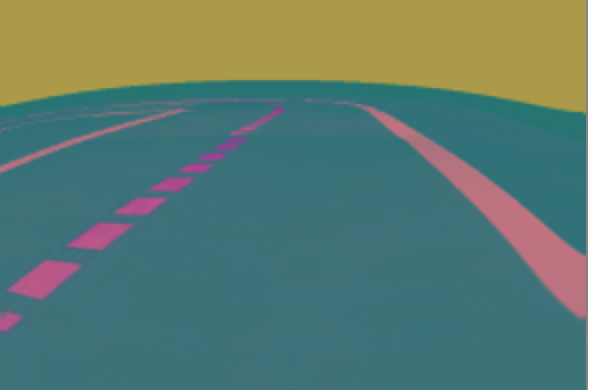
\includegraphics[width=4cm]{sim_data} }}
    \qquad
    \subfloat[\centering Public log data]{{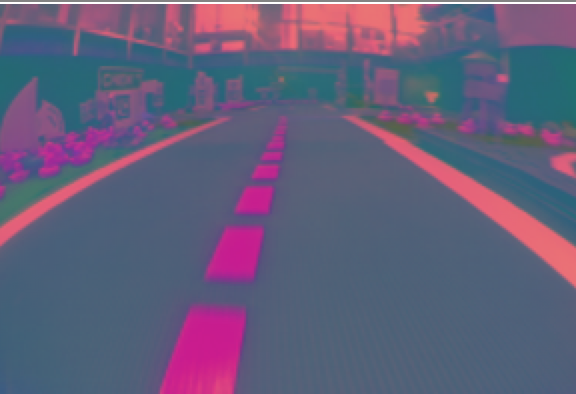
\includegraphics[width=4cm]{log_data} }}
    \qquad
    \subfloat[\centering Custom data]{{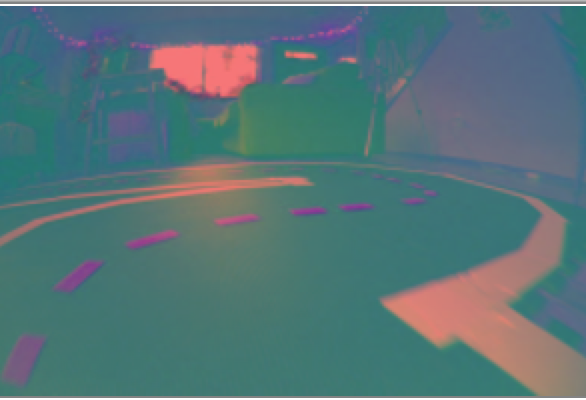
\includegraphics[width=4cm]{custom_data} }}
    \caption{Example frames from the three different data sources used for training. Observations are downsampled 150x200 pixel images.}
    \label{fig:data_examples}
\end{figure}

Ultimately we used two final datatsets. The largest (henceforth ``dataset A") was used for training the initial model and consisted of 58,414 total observation frames with associated controls, this was a mix of simulated data collected from \texttt{gym-duckietown} (50,337 frames) and public real robot data (8,077 frames). The second dataset (henceforth ``dataset B") was used for experimenting with fine tuning our models and consisted of 15,560 total frames, this only contained our custom real robot data.

\subsection{Model Architectures} \label{sec:model_arch}

    Our experiments were focused around two model architectures, the first was an attempt to reproduce results from NVIDIA \cite{DBLP:journals/corr/BojarskiTDFFGJM16} which we named the ``nvidia" model (Figure \ref{fig:model_arch}a). In order to predict two values (linear and angular velocity) two separate instantiations of this model were created with disjoint weights. The only major deviations from the originally published model were the use of leaky rectified linear unit (LeakyReLU) activations and dropout in-between linear layers ($p=0.5$).
    The second architecture used a smaller number of total parameters, shared weights across the convolutional layers, and two outputs preceded by small disjoint linear layers (Figure \ref{fig:model_arch}b). We named the initial version of this model ``modelv0", subsequent experimentation produced a second version ``modelv1" which substituted ReLU activations for LeakyReLU, and added dropout to the final linear layers ($p=0.5$) and the shared convolutional layers ($p=0.1$).

\begin{figure}
    \subfloat[\centering]{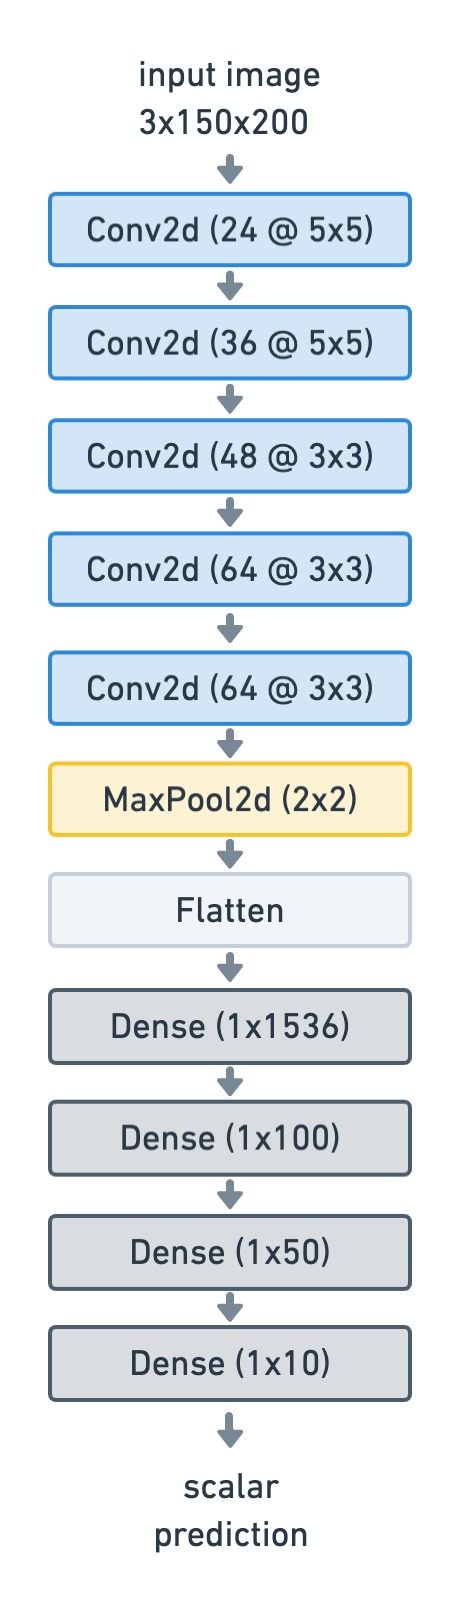
\includegraphics[width=.22\textwidth,keepaspectratio]{nvidia_arch}}
    \subfloat[\centering]{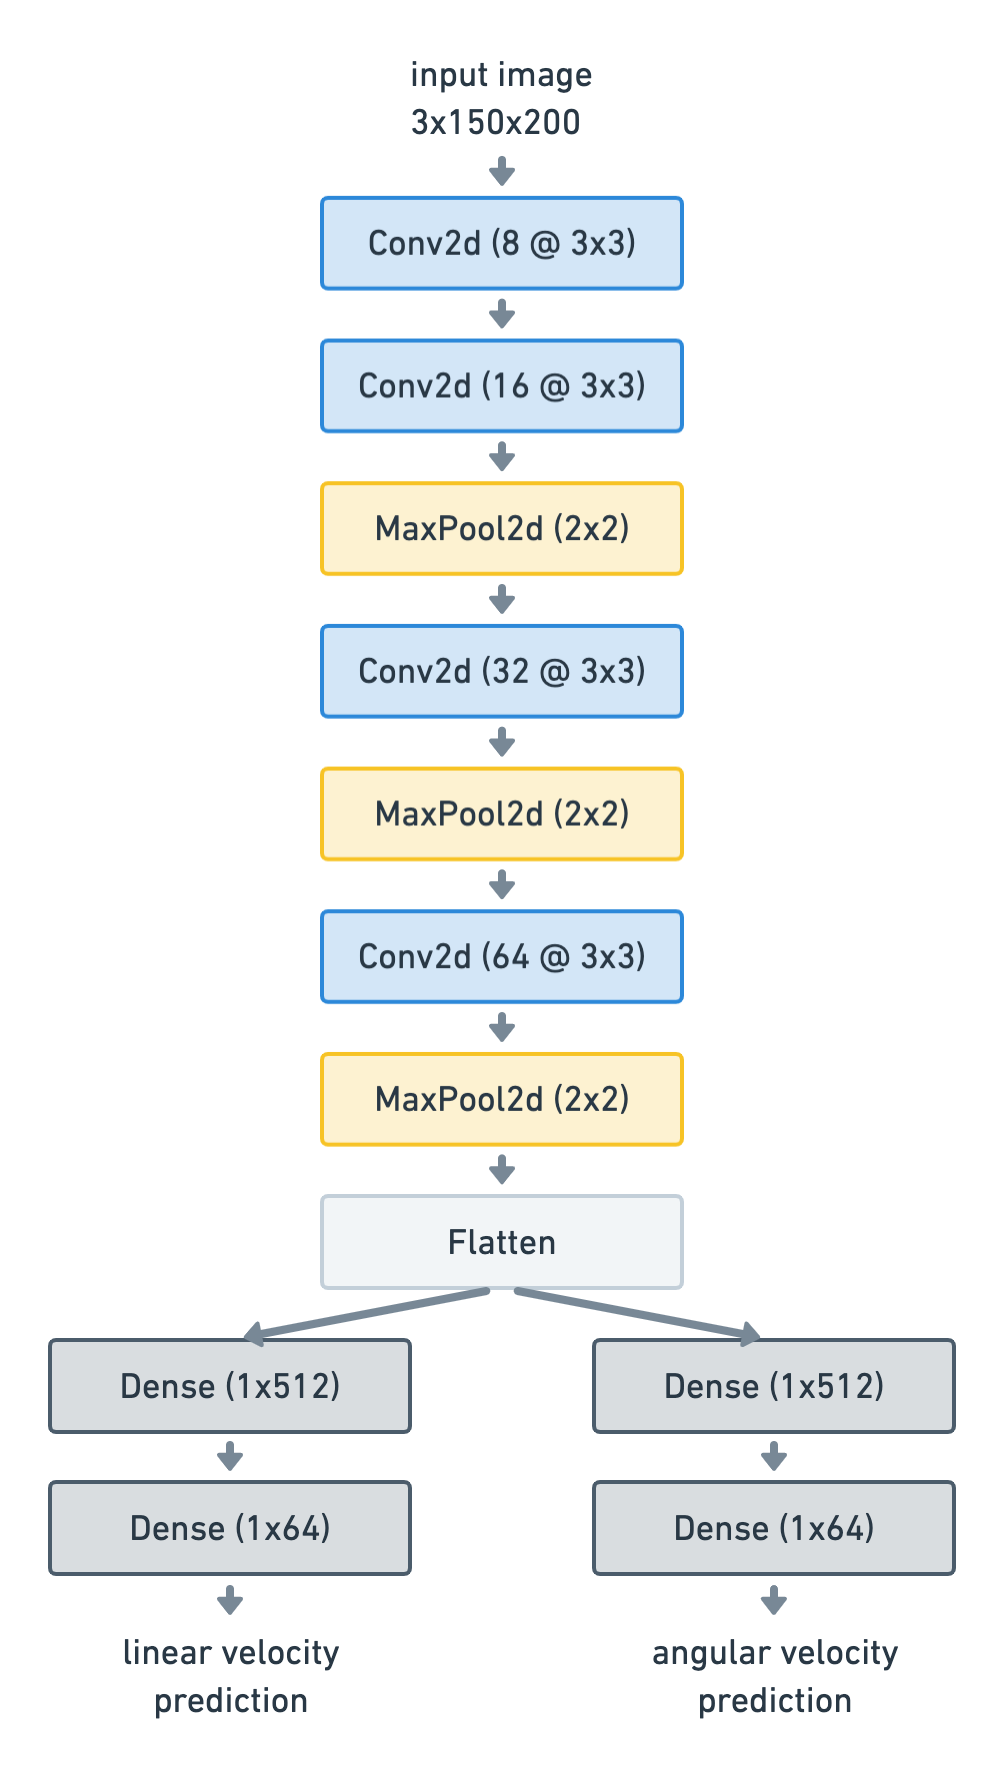
\includegraphics[width=.43\textwidth,keepaspectratio]{dual_cnn_arch}}
\centering
    \caption{Overview of the two primary model architectures evaluated in this work. (a) features a larger number of total parameters and no shared weights, each of the two prediction values retain their own copy of the model (b) uses shared convolutional layers and small linear layers preceding each of the two outputs.}
\label{fig:model_arch}
\end{figure}

\subsection{Training}
All training was done using stochastic gradient descent and mean squared error loss. The models were trained initially on the aggregated dataset (``dataset A") for 200 epochs, results in Figure \ref{fig:training_results}. As the ``nvidia" model did not show promising results during training, it was excluded from further experimentation. Then ``modelv0" and ``modelv1" were fine tuned for 50 epochs using the custom real robot dataset (``dataset B"), results in Figure \ref{fig:fine_tuning_training_results}. A prediction was deemed accurate if the continuous velocity value was within 5\% of the label value.

\begin{figure}
  \centering
  \raisebox{35pt}{\parbox[b]{.1\textwidth}{nvidia}}%
  \subfloat{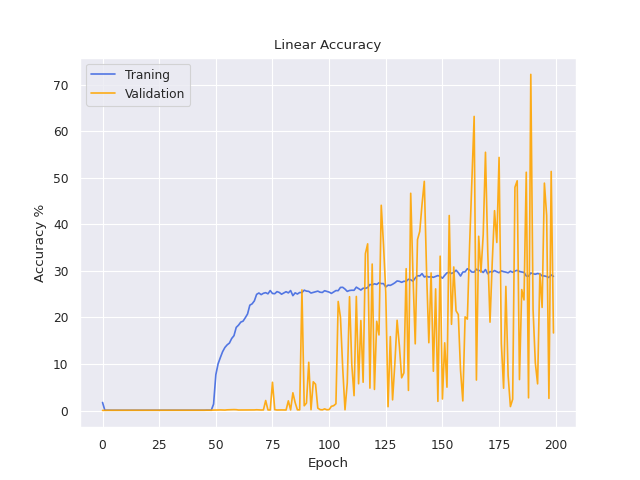
\includegraphics[width=.28\textwidth]{nvidia_linear_accuracy}}\hfill
  \subfloat{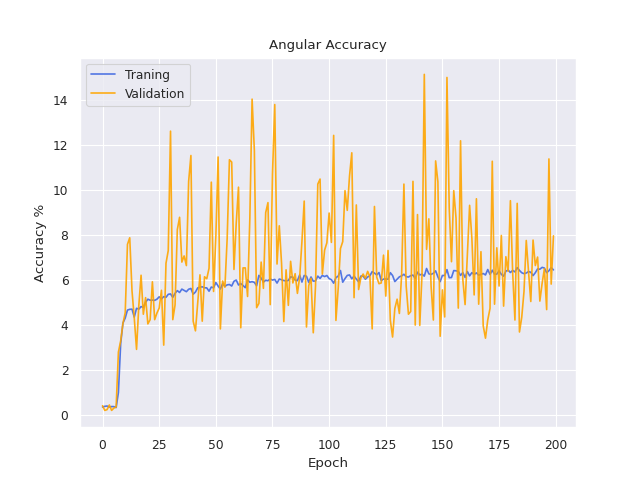
\includegraphics[width=.28\textwidth]{nvidia_angular_accuracy}}\hfill
  \subfloat{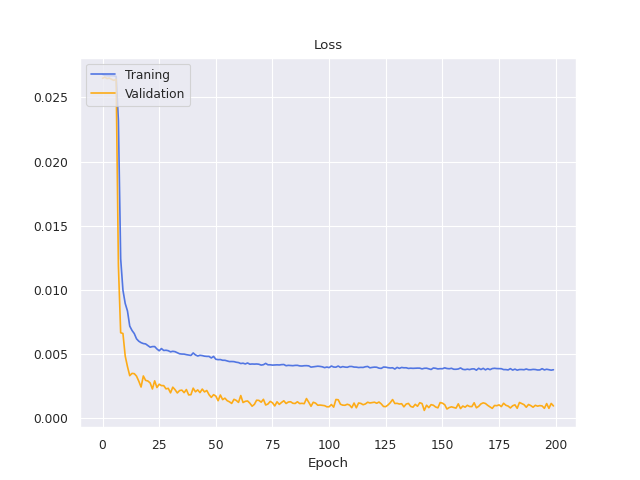
\includegraphics[width=.28\textwidth]{nvidia_loss}}\par
  \raisebox{35pt}{\parbox[b]{.1\textwidth}{modelv0}}%
  \subfloat{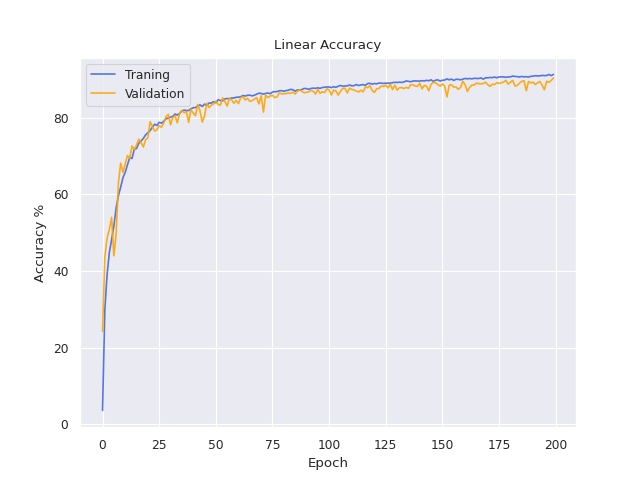
\includegraphics[width=.28\textwidth]{modelv0_linear_accuracy}}\hfill
  \subfloat{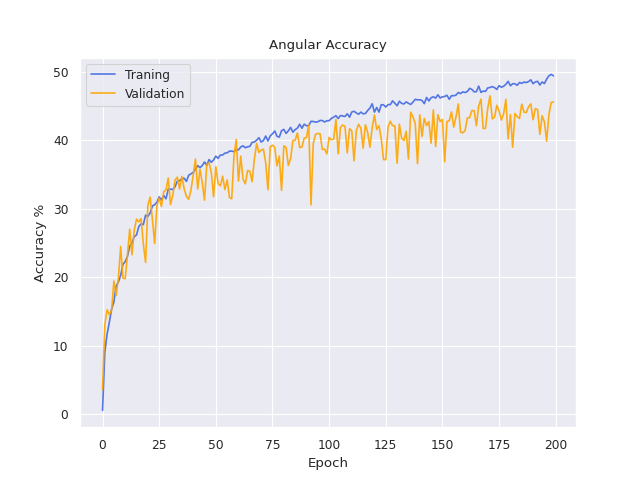
\includegraphics[width=.28\textwidth]{modelv0_angular_accuracy}}\hfill
  \subfloat{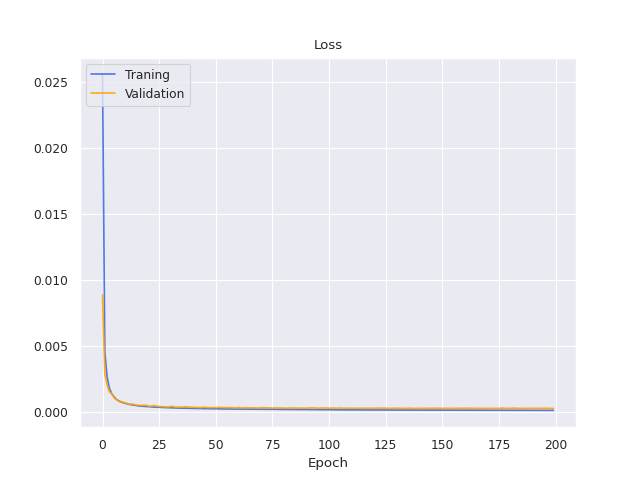
\includegraphics[width=.28\textwidth]{modelv0_loss}}\par
  \raisebox{35pt}{\parbox[b]{.1\textwidth}{modelv1}}%
  \subfloat{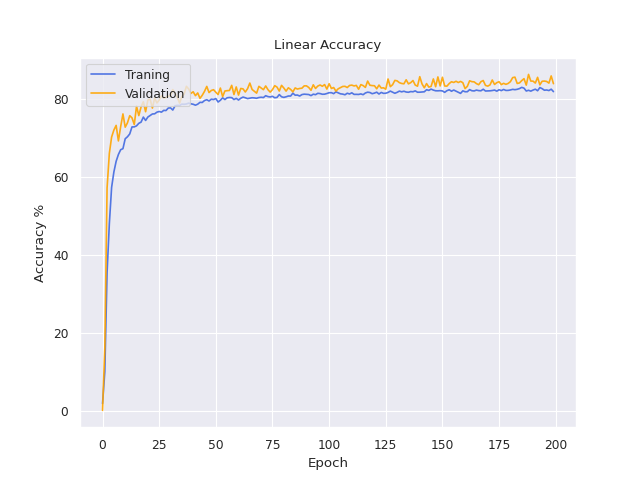
\includegraphics[width=.28\textwidth]{modelv1_linear_accuracy}}\hfill
  \subfloat{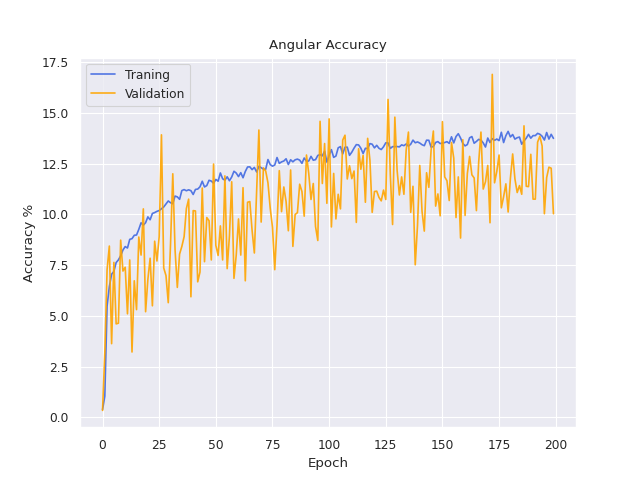
\includegraphics[width=.28\textwidth]{modelv1_angular_accuracy}}\hfill
  \subfloat{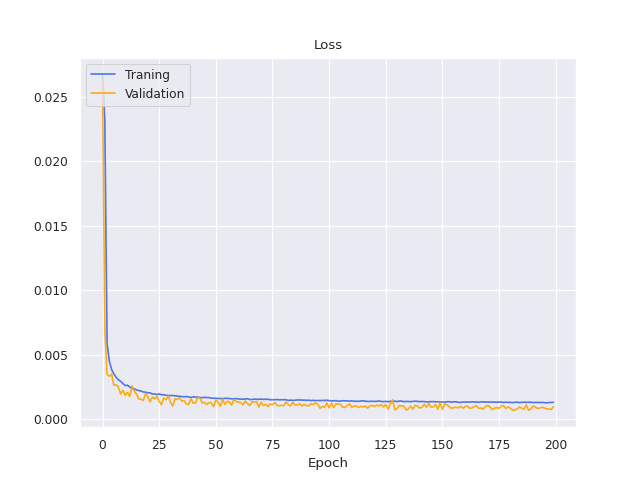
\includegraphics[width=.28\textwidth]{modelv1_loss}}
  \caption{Results from training the three different model architectures on dataset A, showing linear accuracy, angular accuracy, and loss achieved. A prediction was considered correct if the continuous velocity value was within 5\% of the label value.}
  \label{fig:training_results}
\end{figure}

\begin{figure}
  \centering
  \raisebox{35pt}{\parbox[b]{.1\textwidth}{modelv0}}%
  \subfloat{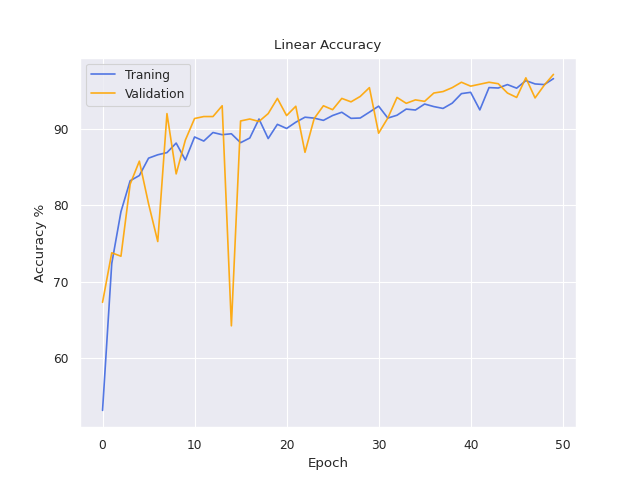
\includegraphics[width=.28\textwidth]{modelv0_200_fine_tuned_cw_ccw_linear_accuracy}}\hfill
  \subfloat{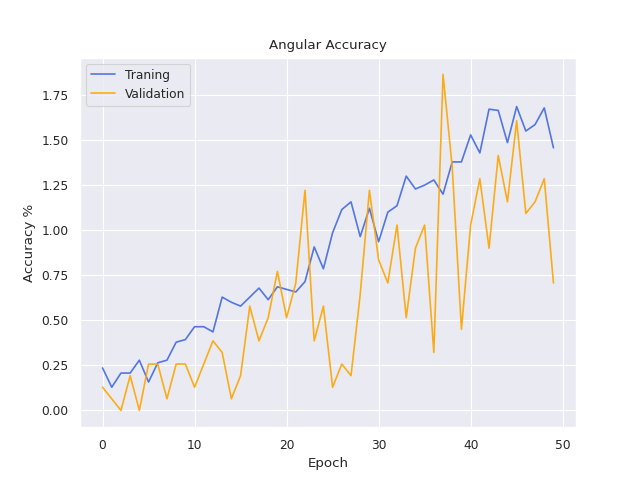
\includegraphics[width=.28\textwidth]{modelv0_200_fine_tuned_cw_ccw_angular_accuracy}}\hfill
  \subfloat{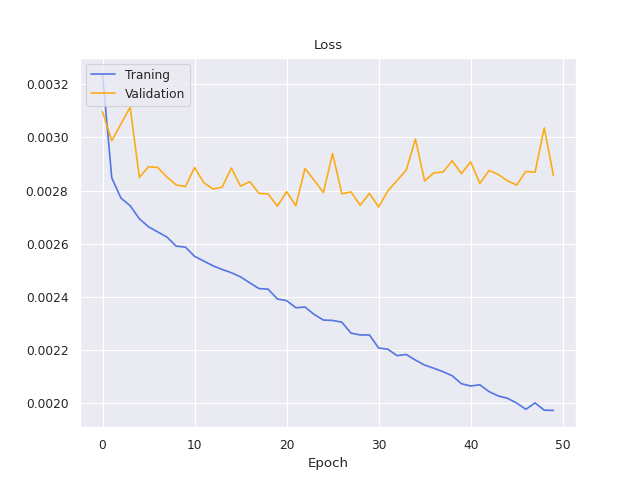
\includegraphics[width=.28\textwidth]{modelv0_200_fine_tuned_cw_ccw_loss}}\par
  \raisebox{35pt}{\parbox[b]{.1\textwidth}{modelv1}}%
  \subfloat{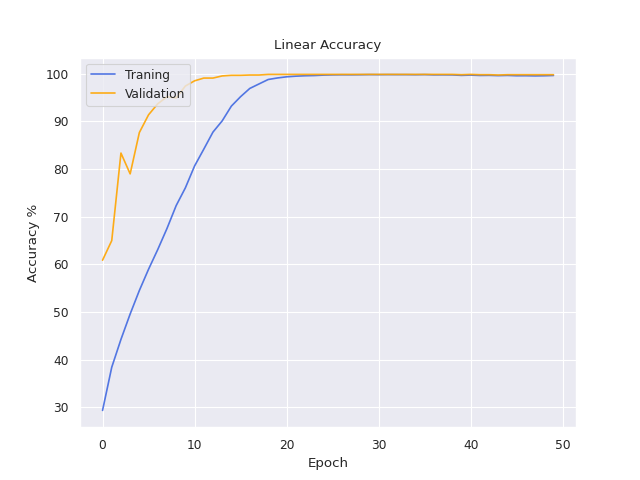
\includegraphics[width=.28\textwidth]{modelv1_200_fine_tuned_cw_ccw_linear_accuracy}}\hfill
  \subfloat{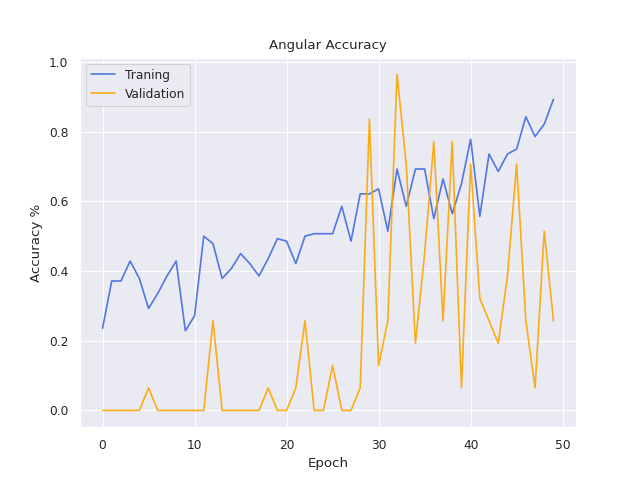
\includegraphics[width=.28\textwidth]{modelv1_200_fine_tuned_cw_ccw_angular_accuracy}}\hfill
  \subfloat{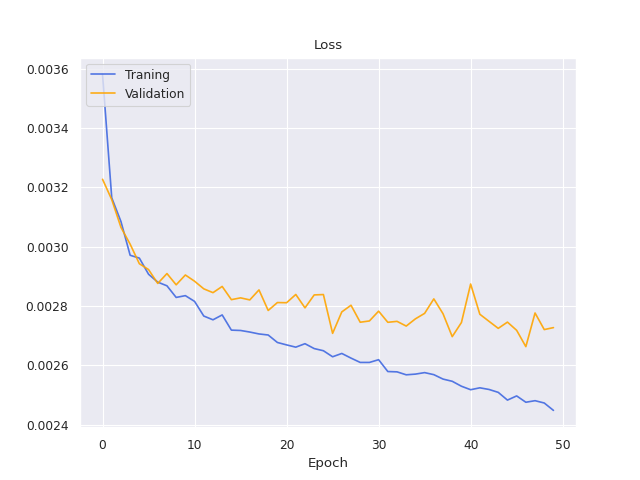
\includegraphics[width=.28\textwidth]{modelv1_200_fine_tuned_cw_ccw_loss}}\par
  \caption{Results from fine tuning the shared weights models on dataset B, showing linear accuracy, angular accuracy, and loss achieved. A prediction was considered correct if the continuous velocity value was within 5\% of the label value. Poor angular accuracy was achieved and training loss on the validation set plateaued quickly.}
  \label{fig:fine_tuning_training_results}
\end{figure}

\section{Performance Evaluations}

\subsection{Simulator and AIDO}

By writing an agent using the agent interface in the AIDO template, we were able to leverage the existing AIDO infrastructure for evaluating in simulation. We submitted all three of our models along with the baseline solution provided by Duckietown to the \texttt{aido-LF-sim-validation} challenge. This evaluates each solution across multiple runs and different maps, providing videos of robot execution in the simulator as well as overhead views of the robot trajectories. Visualization of the trajectories taken for all these models across three maps is shown in Figure \ref{fig:sim_results_original}. We noticed that our models performed roughly equivalent to the baseline solution or did worse.

Following additional experimentation it appeared that the high linear velocity predicted by our models did not allow for sufficient time to make turns, and in general our models had difficulties in applying enough angular velocity to make turns effectively. To counteract this issue we applied hard coded modifications to the predicted linear and angular velocities at each command time step, dividing the predicted velocity by 2 and multiplying the predicted angular velocity by $1.5$. Henceforth these manually modified models are signified as such with the suffix ``*". This modification significantly improved the ability of our agent to navigate, which was our primary objective, even though it was at the cost of decreased travel distance within the 60 second episode length. We also applied this modification to the baseline solution in order to provide a better comparison, these results can be found in Figure \ref{fig:sim_results_modified}.

Simulation results for the fine-tuned models were very poor, performing worse than the original unmodified models even. Visualizations of these results are not included for brevity, but real robot results are discussed below.

\begin{figure}
    \centering
    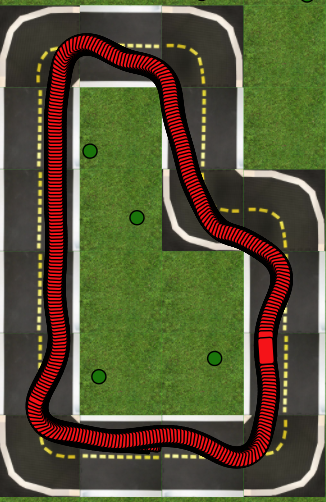
\includegraphics[width=.23\textwidth]{sim_baseline_0}
    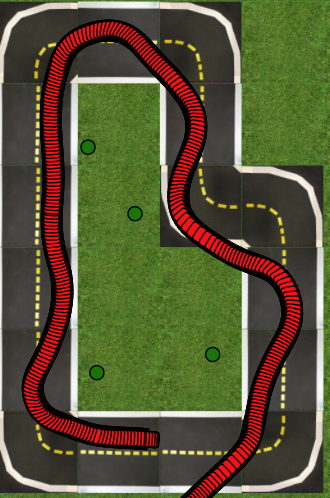
\includegraphics[width=.23\textwidth]{sim_nvidia_0}
    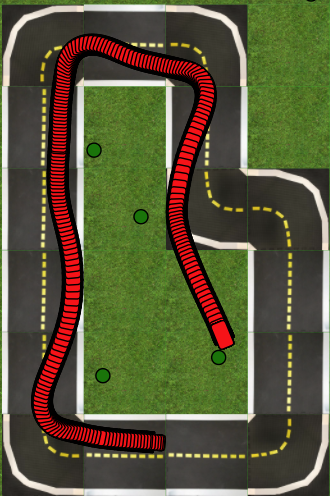
\includegraphics[width=.23\textwidth]{sim_v0_0}
    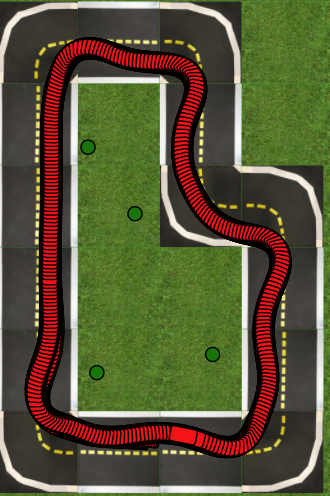
\includegraphics[width=.23\textwidth]{sim_v1_0}

    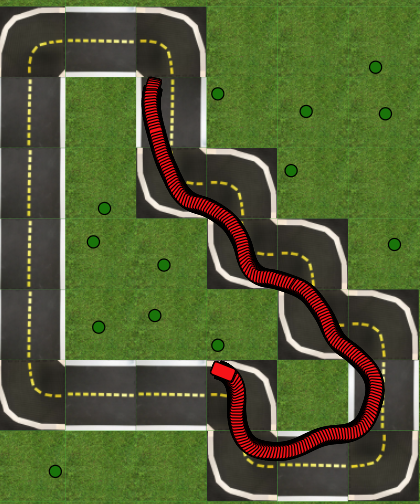
\includegraphics[width=.23\textwidth]{sim_baseline_1}
    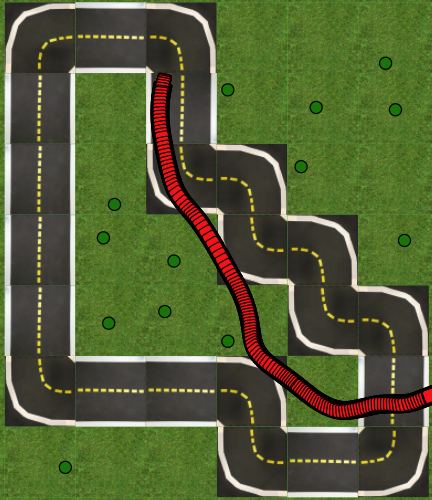
\includegraphics[width=.23\textwidth]{sim_nvidia_1}
    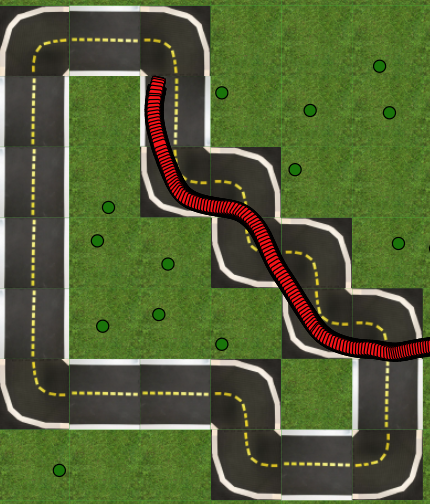
\includegraphics[width=.23\textwidth]{sim_v0_1}
    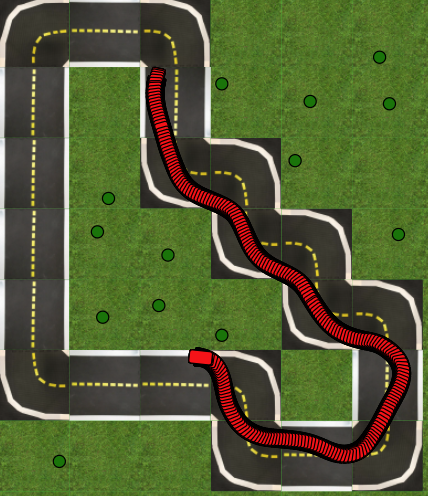
\includegraphics[width=.23\textwidth]{sim_v1_1}

    \subfloat[baseline]{
        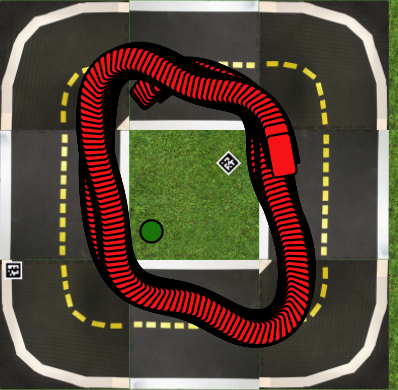
\includegraphics[width=.23\textwidth]{sim_baseline_2}
    }
    \subfloat[nvidia]{
        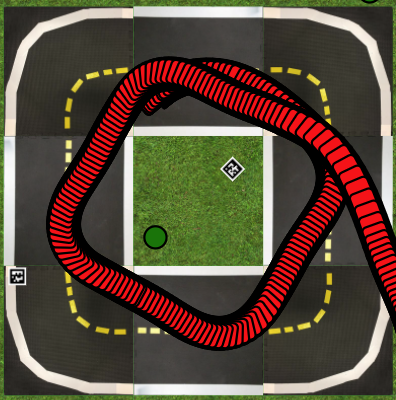
\includegraphics[width=.23\textwidth]{sim_nvidia_2}
    }
    \subfloat[modelv0]{
        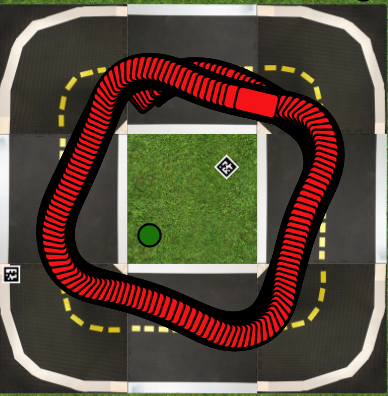
\includegraphics[width=.23\textwidth]{sim_v0_2}
    }
    \subfloat[modelv1]{
        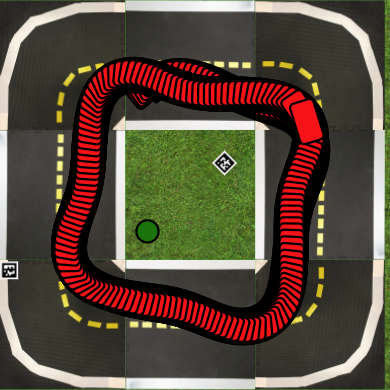
\includegraphics[width=.23\textwidth]{sim_v1_2}
    }
    \caption{Robot trajectories in simulation on three different maps for the baseline solution (a) and each of the evaluated models (b-d).}
  \label{fig:sim_results_original}
\end{figure}

\begin{figure}
    \centering
    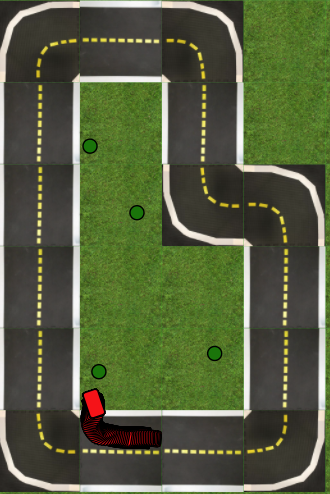
\includegraphics[width=.23\textwidth]{sim_baseline_star_0}
    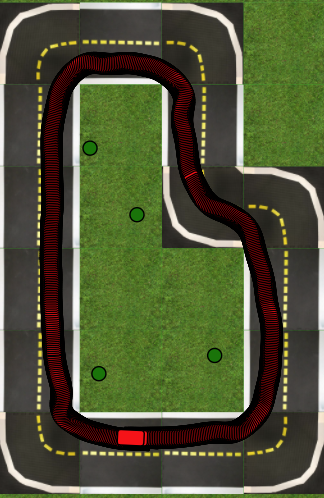
\includegraphics[width=.23\textwidth]{sim_nvidia_star_0}
    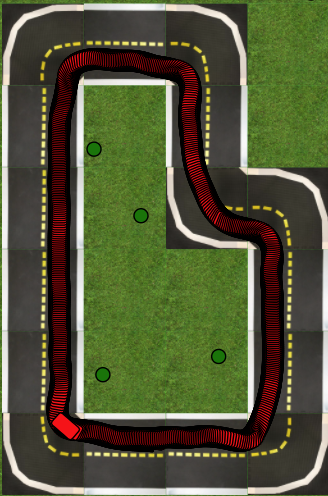
\includegraphics[width=.23\textwidth]{sim_v0_star_0}
    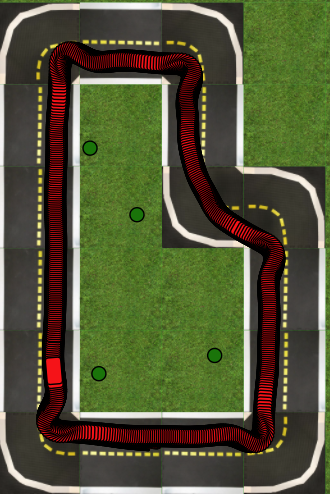
\includegraphics[width=.23\textwidth]{sim_v1_star_0}

    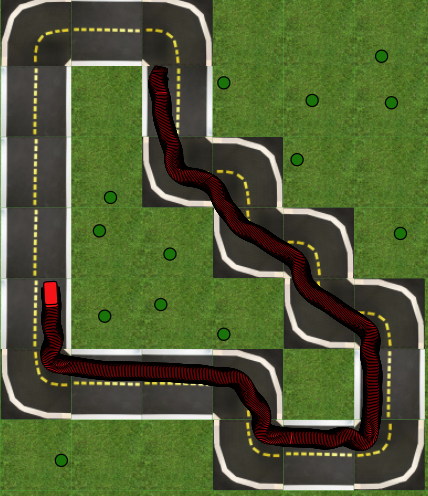
\includegraphics[width=.23\textwidth]{sim_baseline_star_1}
    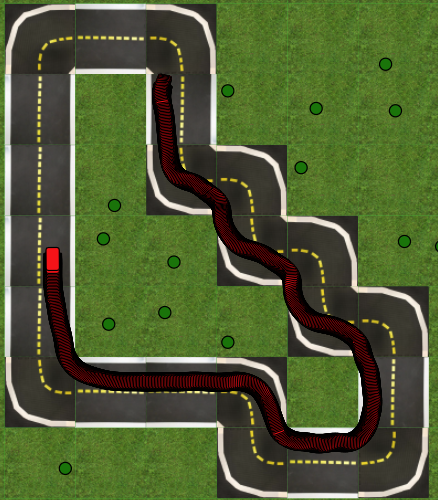
\includegraphics[width=.23\textwidth]{sim_nvidia_star_1}
    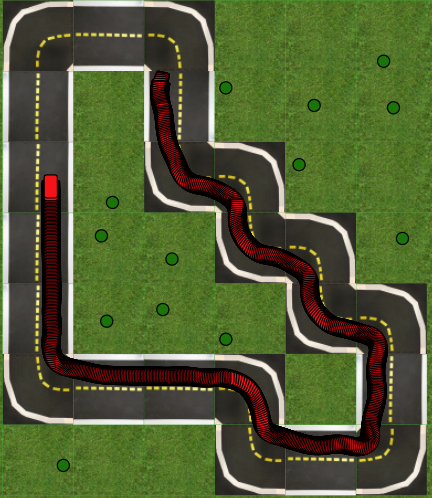
\includegraphics[width=.23\textwidth]{sim_v0_star_1}
    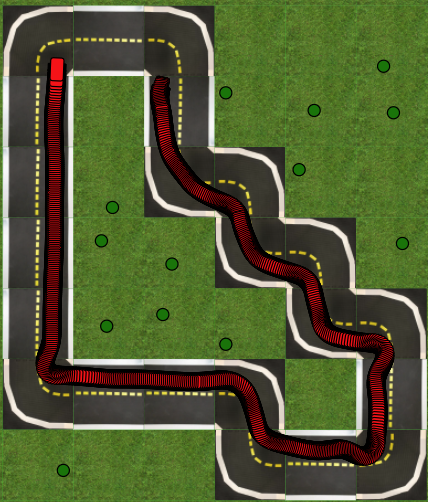
\includegraphics[width=.23\textwidth]{sim_v1_star_1}

    \subfloat[baseline*]{
        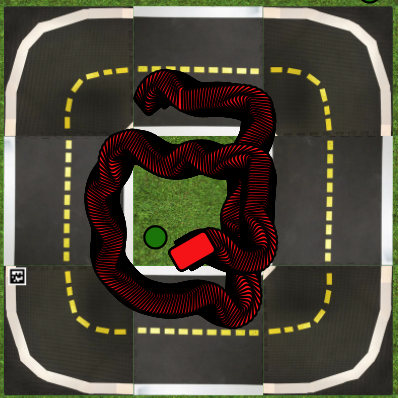
\includegraphics[width=.23\textwidth]{sim_baseline_star_2}
    }
    \subfloat[nvidia*]{
        \includegraphics[width=.23\textwidth]{sim_nvidia_star_2}
    }
    \subfloat[modelv0*]{
        \includegraphics[width=.23\textwidth]{sim_v0_star_2}
    }
    \subfloat[modelv1*]{
        \includegraphics[width=.23\textwidth]{sim_v1_star_2}
    }
    \caption{Robot trajectories in simulation on three different maps for the baseline solution (a) and each of the evaluated models (b-d), in all cases the solutions were manually modified to apply a linear transformation of the predicted velocity values.}
  \label{fig:sim_results_modified}
\end{figure}

\subsection{Real World}

Having previously determined in simulation that the manually modified models (``nvidia*", ``modelv0*", ``modelv1*") performed best, we expected this result to be true during real robot evaluation as well. All initial evaluations were done on map2 (Figure \ref{fig:maps}b) and from these we determined that ``modelv1*" was the overall best performing model, so it was evaluated on the other maps as well.

The following videos contain results from testing all three models along with the baseline solution on map2:
\begin{itemize}
    \item original models: \url{https://youtu.be/j7rHbaK74h8}
    \item modified models: \url{https://youtu.be/6s80amO3GV8}
\end{itemize}

\subsubsection{Fine Tuning}

Consistent with the accuracy obtained during training and lack of ability to decrease validation set loss when performing fine tuning (Figure \ref{fig:fine_tuning_training_results}), real robot performance was much worse with this additional training, see \url{https://youtu.be/v5AOjATDAyU}. This is not altogether surprising though given that poor quality of the human driver controls used to create the custom dataset. It was simply too difficult to drive the robot even as a human given the coarse grained tools provided for user input and the overall quality and reliability of the robot. During human driving there were consistently moments where the robot seemed to drift off and execute some control the human did not apply. These factors likely contributed to a noisy dataset that did not improve the performance of our system.

\subsubsection{Generalization}

In order to evaluate the ability of our best performing model ``modelv1*" to generalize to other maps it was tested alongside ``baseline*" on the remaining maps (see below). In general the results were consistent with performance on map2 with the caveat that our solution could not handle right turns. This is likely an issue with our dataset having not enough examples of right turns and hence the robot was unable to use prior examples to successfully navigate this situation.

\begin{itemize}
    \item map1: \url{https://youtu.be/jYgHov8mpX4}
    \item map3: \url{https://youtu.be/ALZrHWevRJ4}
    \item map4: \url{https://youtu.be/Oodr0QcEKJM}
    \item map5: \url{https://youtu.be/zt69aAOWHX4}
\end{itemize}

\section{Potential Future Improvements}
\begin{enumerate}
    \item As explained in prior sections, one limitation faced was the difficultly in collecting good real robot data. Possibly one way to have circumvented this was to use the duckiebot's Xbox controller interface for human driving, assuming that this input possibly has better fine grained control.
    \item As observed in our agent's inability to generalize to certain maps, we had a dearth of data with right hand turns. Improving our dataset to include more diverse situations would likely improve real world performance.
    \item In general issues with the robot caused limitations in our groups ability to properly evaluate our agents. One group member's robot had consistent issues with keeping its wheel on and rendered him unable to use his robot in a meaningful way. The use of more robust robot components would certainly improve the ability to iterate during experimentation and also have a system less subject to control noise.
    \item We suspected that performance at inference time might have been a bottleneck for our system. Possibly this is one reason that introducing a hard coded linear velocity reduction improved performance, by allowing time to do inference on observations corresponding to turn taking. A potential place to look for performance improvement would be to either quantize our PyTorch model to speed up CPU-based inference, or to adapted our system to use the onboard GPU on the Jetson Nano. Despite some effort in trying to adapt the duckietown software stack to use the GPU, the containerized software system was unable to detect the on-board GPU and hence we could not leverage it.
    \item We also believe that using a recurrent network model has the potential to improve performance. Although our data input is actually video, we treated it as isolated image frames and lost the ability to leverage prior observations in making predictions.
\end{enumerate}

\bibliographystyle{alpha}
\bibliography{paper}

\end{document}
